\clearpage
\chapter{Der Industriezweig Uhr}
\section{Geschichtliches zur Uhrindustrie}
Die Schweiz ist derzeit das Land mit den meisten Uhrenexporten. Gemessen an den Exporten ist die Uhrenindustrie innerhalb der Schweiz jedoch nur die drittgrößte Industrie. Weltweit gefolgt wird die Schweiz Hongkong und China.\\ 
In den 1970er und 1980er Jahren erhielt die klassische schweizer Uhrenindustrie Konkurrenz durch die Entstehung der elektrischen Uhren und den asiatischen Markt. Nachdem sie sich bis 2015 wieder etwas erholen konnte und die Exporte von 4,3 Milliarden Franken im Jahr 1986 auf 21,5 Milliarden im Jahr 2015.\\ 
Mittlerweile schaffen es vor allem die Großmarken, sich gegen die neue Konkurrenz der Smart Watches durchzusetzen, indem sie entweder hochwertige Luxusuhren herstellen, die als Schmuckstück und Statussymbol dienen oder indem sie selbst Smart Watches entwickeln.

\section{Marktsituation}
Der weltweite Uhrenmarkt wird nur von wenigen Länder beherrscht. Die Schweiz und China stechen dabei hervor. China ist mengenmässig der weltweit größte Uhrenproduzent. Chinesische Uhren sind dabei hauptsächlich im niedrigen Preissegment angesiedelt. Im hochwertigen Segment ist die Schweiz hingegen mit Abstand Marktführer. Auf Basis der Stückzahlen macht die Schweiz nur rund 2.5\% der globalen Produktion aus. Wertmässig dagegen ist die Schweiz mit Abstand führendes Uhrenexportland. Auf Unternehmensebene sind mit der Swatch Group, Richemont und Rolex drei Schweizer Betriebe klare Weltmarktführer. Zusammen vereinen die drei Konzerne etwa 30\% bis 50\% des globalen Uhrenumsatzes. 94\% des Schweizer Uhrenexportumsatzes in Höhe von 17 Milliarden EURO wurde 2012 mit fertigen Kleinuhren erzielt. Der hohe Umsatz wird mit vergleichsweise wenigen, aber teuren Uhren erwirtschaftet.

Die weltweite Uhrenindustrie wird hauptsächlich von folgenden Ländern beherrscht: Schweiz, Hongkong, China, Deutschland, Frankreich, Singapur, Italien, Japan, die USA und Großbritannien. Diese genannten Länder machen über 90\% der globalen Exporte von Uhren aus. Deutlich über 90\% Prozent aller aus China exportierten Uhren sind Quarzuhren. In der Schweiz stellen solche Uhren unter 20\% des Exportumsatzes dar. Mit Citizen, Seiko und Casio gehören neben Schweizer Firmen auch drei Japanische Konzerne mit ihren Umsätzen zu den wichtigsten Unternehmen auf dem Weltmarkt der Uhren.

Wir bieten daher schwerpunktmäßig für Schweizer Uhren mit ihrem hohen Anteil an mechanischen und somit besonders reparaturintensiven Zeitmessern Reparaturen und Serviceleistungen an.

\begin{figure}[!h]
	\centering
	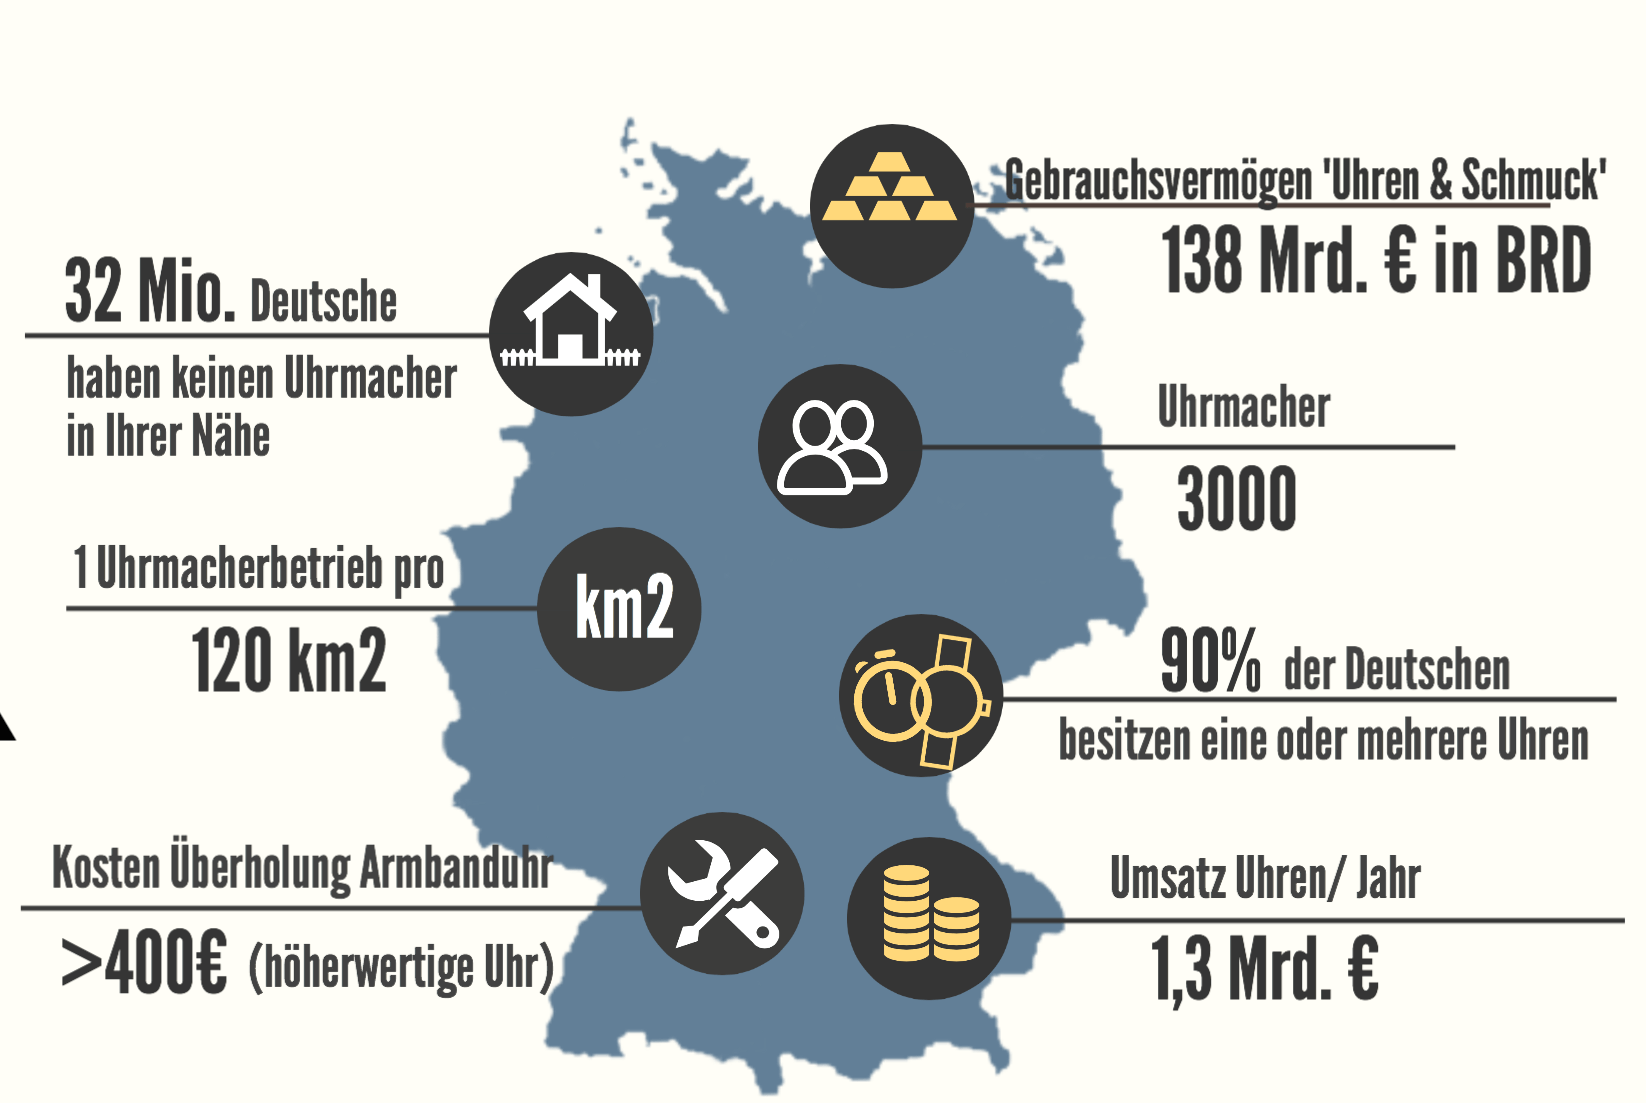
\includegraphics[scale=0.2]{statistiken/uhrenmarkt_info.png}
	\label{fig:abb1}
	\caption{Piktorgramm des Uhrenmarkts} 
\end{figure}

